

    The following illustrates the class definition for an inbuilt function,
    in this case {\bf sin()} -
    
    \begin{lstlisting}[gobble=4, language=java]
        package threepl.funcs;

        import threepl.exceptions.ExEx;
        import threepl.exec.Val;
        import threepl.nodes.NodeList;
        import threepl.parser.Constant;
        import threepl.parser.SrcLoc;

        /**
         * An inbuilt function to get the sine.
         */
        public class SinFunc extends InbuiltFunc implements Constant {
            .
            .
            .
        }
    \end{lstlisting}

    For inbuilt modules and procedures the class definition is similar to that
    for functions -
        
    \begin{lstlisting}[gobble=4, language=java]
        package threepl.procs;

        import threepl.exceptions.ExEx;
        import threepl.exec.Ref;
        import threepl.exec.Val;
        import threepl.nodes.NodeList;
        import threepl.parser.Constant;
        import threepl.parser.SrcLoc;
        import threepl.parser.Functions;


        /**
         * An inbuilt procedure to scan a string converting delimited fields to types specified
         * by a format string.
         */
        public class SscanfProc extends InbuiltProc implements Constant {
            .
            .
            .
        }
    \end{lstlisting}
    
    For procedures there is an optional constructor, e.g. -
    
    \begin{lstlisting}[gobble=4, language=java]
        public SscanfProc () {
            allowed_as_param = false;
            check_null_input_args = true;
            check_null_output_args = true;
            target_inline = false;
        }
    \end{lstlisting}
    
    These boolean variables are all declared and initialised in
    InbuiltProc.java and their functions are as follows -
    
    \blist
    \item allowed\_as\_param - true if the procedure is allowed as a
        parameter-creation procedure, i.e. can appear as a parameter in
        a function module or procedure definition.
    \item check\_null\_input\_args - if true null input arguments will throw
        an exception
    \item check\_null\_output\_args - if true null output arguments will throw
        an exception
    \item target\_inline - if true the procedure generates in-line target code
    \blend
    
    These booleans are set false by the super class but assigning them here
    improves readability. The null argument detection avoids the need in many
    cases for the module or procedure to explicitly check if an argument is null.
    Some procedures however accept null arguments and hence do not want this test
    enabled.
    
    There are two additional member variables, applicable to both modules
    and procedures -
    
    \begin{lstlisting}[gobble=4, language=java]
        public TreeMap<String,Integer>  ipnames;
        public TreeMap<String,Integer>  opnames;
    \end{lstlisting}
    
    which are null by default. These maps can contain identifiers to be
    associated with the module or procedure input and output parameters so that
    the module or procedure can be passed arguments either by position or by
    parameter=argument. If these maps are null then only the usual 
    parameter/argument association by position is available. The map keys contain
    the parameter identifiers and the associated integers are the parameter
    position. The maps need not contain all parameters as it is often convenient
    to pass some initial mandatory arguments by position.
    
    When a parameter name map has been provided the parameter=name arguments
    will be re-arranged in the argument list so that the module or
    procedure only sees arguments in the correct order. Note that for many
    modules and procedures null arguments are allowed in the call and in addition
    the argument re-arrangement for parameter=argument entries may also
    introduce null arguments.
    
    Inbuilt modules, procedures and functions are listed in maps in
    InbuiltMods.java, InbuiltProcs.java and InbuiltFuncs.java e.g. -
    
    \begin{lstlisting}[gobble=4, language=java]
        public InbuiltProcs () {
            procs = new TreeMap<String, InbuiltProc>();

            procs.put("addmodeattribute", new AddModeAttributeProc());
            .
            .
            .
        }
    \end{lstlisting}
    
    Here the map key is the identifier by which the module, procedure
    or function is called and the associated entry is the actual
    module, procedure or function. The identifiers are lower case
    and the actual classes are camel case with "Mod", "Proc" or "Func"
    appended, but this is only a convention.    

    The calling procedure for inbuilt modules, procedures and functions
    is the same with the exception that functions do not have output
    parameters.
    
    Functions have a getVal() method to return the function value.
    For example the {\bf sin()} function -
    
    \begin{lstlisting}[gobble=4, language=java]
        public Val getVal (NodeList args) {
            SrcLoc  loc = args.getCallLoc();

            if (args.size() != 1)
                throw new ExEx("sin() - must have one argument", loc);
            .
            .
            .
    \end{lstlisting}
    
    class {\bf NodeList} is a linked list of nodes in the compiled code
    tree. Variable {\bf args} contains the list of arguments of the
    function call.
    
    Class {\bf SrcLoc} contains source code file name, line number and
    character column. {\bf doc} is assigned the function call location.
    
    The size of {\bf args} is checked to ensure that the number of arguments
    provided is correct.
    
    Modules and procedures have an execute() method.
    For example the procedure {\bf sscanf()} -
    
    \begin{lstlisting}[gobble=4, language=java]
        public void execute (
            NodeList    inargs, 
            NodeList    outargs, 
            boolean     toplevel
    ) {
        SrcLoc      loc = inargs.getCallLoc();
        if (inargs.size() != 2)
            throw new ExEx("sscanf() must have two input arguments", loc);
        if (outargs.size() == 0)
            throw new ExEx("sscanf() must have one or more output arguments", loc);        
        .
        .
        .
    \end{lstlisting}
    
    The signature is similar for a module except that the {\bf toplevel}
    parameter is not present.
    
    Where a procedure is allowed to be called to create a parameter in a
    module, procedure or function definition the call to the procedure
    is more complicated, e.g. for inbuilt procedure {\bf int()} -
       
    \begin{lstlisting}[gobble=4, language=java]
        public IntProc () {
            allowed_as_param = true;
            check_null_input_args = true;
            check_null_output_args = false;
            target_inline = false;
            allowed_attributes = true;
        }

        /**
         * Execute the variable declaration procedure int().
         */
        public ArrayList<Var> execute (
            NodeList            inargs,
            NodeList            outargs,
            ArrayList<String>   names,
            RefOrVal            par_arg,
            int[]               dim_des,
            boolean             is_input,
            boolean             is_output
        ) {
            .
            .
            .
        }
    \end{lstlisting}
    
    The extra member variable {\bf allowed\_attributes} is true to indicate that
    the arguments to the procedure can contain attributes. Attributes are passed
    as attribute=value. Some must be processed by the module or procedure itself.
    In the case of procedures {\bf clock()}, {\bf input()} and {\bf output()}
    attributes are processed by 3PL code whenever the procedure is called via a
    3PL call-back procedure. If this variable is true then a mixture of
    parameter=argument and attribute=value arguments will be resolved. Arguments
    to the module or procedure will appear in the argument list as simple
    positional arguments as a result of the identifier resolution described
    above. Any that are not recognised are assumned to be attribute=value and
    these will be appended as additionak arguments following the positional
    arguments and will be class KeyMatchNode. These trailing attributes must be
    processed by the module or procedure.
    
    The arguments to execute() are -
      
    \blist
    \item inargs is a list of input argument tree nodes
    \item outargs is a list of output argument tree nodes
    \item names is a list of identifiers evaluated via method
            getIdents() prior to calling execute()
    \item par\_arg is an argument passed to this variable as a parameter in
            a call
    \item dim\_des is a dimensional description for a compound constant
            argument or is null - it must be null here!
    \item is\_input is true if this variable is the input parameter
            for a module, procedure or function
    \item is\_output is true if this variable is the output parameter
            for a module or procedure 
    \blend
    
    The procedure must return an ArrayList<Var> containing the variable(s).

    The call arguments are supplied separately by {\bf inargs} and {\bf outargs}.
    The boolean argument {\bf toplevel} is only present for procedures, not
    modules, and is true if the procedure call is not nested within a
    target control structure wuch as a par{}, seq{}, sync{}, when{} etc.
    Its value is only used in the inbuilt procedure useclock() (UseCLockProc.java)
    to ensure that changes to the clock domain in use do not occur within target
    code structures.
    
    As with function calls the location of the call is assigned to {\bf loc}.
    The number of input and output arguments is checked.
    
    A procedure may generate in-line code (a module cannot). This means that it
    must insert the generated code into the current execution thread. Such a
    procedure has member variable {\bf target\_inline} true. The call to such a
    procedure has a yet more complicated signature -

    \begin{lstlisting}[gobble=4, language=java]
        public void execute (
            NodeList            inargs,
            NodeList            outargs,
            TDEVar              esig,
            ArrayList<TDEVar>   startl, 
            ArrayList<TDEVar>   finishl,
            QueueRefs            queues,
            boolean             skipexecp,
            TDEVar              pri_in,
            TDEVar              pri_out
        ) {
            .
            .
            .
        }
    \end{lstlisting}

    \blist
    \item inargs is a list of input argument tree nodes
    \item outargs is a list of output argument tree nodes
    \item esig is an exception/restart signal, or null
    \item startl is a list of start signals for target statements below this node
    \item finishl is a list of finish signals for target statements below this
            node
    \item queues returns all the queue availability signals accumulated from
            code below
    \item skipexecp is true if a previous sync makes a queue availability
            wait unnecessary
    \item pri\_in is an optional input signal to a priority encoder
    \item pri\_out is an optional output signal from a priority encoder
    \blend
    
    A procedure may generate a single target executable statement. That statement
    may of course contain nested statements within control structures. Nested
    target statements are common in user-defined procedures but do not occur at
    present in inbuilt procedures.


    \section{functions with immediate mode arguments and return value}
    
        The function code fetches arguments by using the {\bf getVal()} method,
        for example -
        
        \begin{lstlisting}[gobble=8, language=java]
            Val val = args.getVal(0);
        \end{lstlisting}

        for the first argument (0). This is returned as class {\bf Val} which
        is a universal class for both immediate and target expression values.
        The mode and type of the value can be tested by -

        \begin{lstlisting}[gobble=8, language=java]
            if (val.getMode() != Mode.IMMEDIATE)
                throw new ExEx("sin() argument not immediate mode", loc);
            if (val.getPrimType() != Ptype.FLOAT)
                throw new ExEx("sin() argument not a float", loc);
        \end{lstlisting}

        For immediate mode arguments the value can be extracted.
        by one of the methods -

        \blist
        \item getSingleEval(SrcLoc) - an enumerated type value as an EnumConst class
        \item getSingleFileVal(SrcLoc) - a file as a FileDesc class
        \item getSingleFval(SrcLoc) - a floating point value as a double
        \item getSingleIval(SrcLoc) - an integer as a long
        \item getSingleLISTval(SrcLoc) - a list as an ArrayList<Val>
        \item getSingleLval(SrcLoc) - a logical value as a boolean
        \item getSingleMAPval(SrcLoc) - a map as a TreeMap<String,Val>
        \item getSinglePval(SrcLoc) - a pointer value as a Ref class
        \item getSingleSval(SrcLoc) - a string
        \item getSingleTval(SrcLoc) - a type as class Type
        \blend
        
        For arrays and structs a member can be extracted by
        val.getVal(i) where i is the index into the array or struct.
        For an array {\bf val} will contain a one-dimensional representation
        of the data and the offset must be determined from the subscripts
        and dimensions. For a struct the data types will usually be mixed.
        The data types for either will be those listed above for single
        values.
        
        The function return value must be class Val, for example for
        sin() -
        \begin{lstlisting}[gobble=8, language=java]
            double  f = val.getSingleFval(loc);
            return(new Val(Math.sin(f), loc));
        \end{lstlisting}
        
        Class {\bf Val} has a number of constructors for immediate mode types -
        
        \blist
        \item new Val(boolean, SrcLoc) - a boolean (type"log")
        \item new Val(long, SrcLoc) - an integer (type "uint" or "int")
        \item new Val(double, SrcLoc) - a floating point value (type "float")
        \item new Val(String, SrcLoc) - a string (type "str")
        \item new Val(Type, SrcLoc) - a type (stypw "type")
        \item new Val(Object[], String, SrcLoc) - an array
        \item new Val(Object[], Type[], WordSpec, Var, SubFieldList, SrcLoc) -
                struct
        \blend

    \section{functions with target mode arguments or return value}
    
        An example where both the single input argument is target mode and
        the return value is also target mode is queueisempty() -
    
        \begin{lstlisting}[gobble=8, language=java]
            package threepl.funcs;

            import threepl.codegen.TDEVar;
            import threepl.exceptions.ExEx;
            import threepl.exec.Queue;
            import threepl.exec.Val;
            import threepl.exec.Var;
            import threepl.exec.Var.IDtype;
            import threepl.nodes.NodeList;
            import threepl.parser.Constant;
            import threepl.parser.SrcLoc;

            /**
             * An inbuilt function to get a target value which is true if a
             * synchronous queue is empty.
             */
            public class QueueIsEmptyFunc extends InbuiltFunc implements Constant {

                /**
                 * Calling interface for the function.
                 * @param   args is a list of argument tree nodes
                 * @return  the number of free spaces in the queue
                 */
                public Val getVal (NodeList args) {
                    SrcLoc  loc = args.getCallLoc();

                    if (args.size() != 1)
                        throw new ExEx("queueisempty() must have a single argument", loc);

                    Val     val = args.getVal(0);
                    Var     var = val.getVar();
                    if (var == null)
                        throw new ExEx("queueisempty(): argument is not a variable", loc);
                    if (var.getMode() != Mode.QUEUE)
                        throw new ExEx("queueisempty(): '" + var.getID(IDtype.CHAIN) + "' is not a queue variable", loc);

                    TDEVar  t = ((Queue)var).getQueueEmpty(loc);

                    Val oval = new Val(null, Mode.VALUE, t, loc);
                    oval.addOVar(var);
                    return(oval);
                }
            }
        \end{lstlisting}
        
        This follows the examples illustrated previously but the argument
        is now mode {\bf queue}, not mode {\bf immediate}. {\bf val} is
        extracted from the first (only) input argument as before but now
        the argument is assumed to be a variable which is accessed by
        {\bf Var var = val.getVar()}. If the argument is not a variable
        then this will be null and an exception is thrown. The mode is
        then checked and if not mode {\bf queue} an exception is thrown.
        
        The empty state of the queue is detected by method
        {\bf getQueueEmpty(loc)}. Since this is a method specific to class
        Queue the variable {\bf var} of class {\bf Var} must be cast to class Queue.
        The result returned is a signal indicating if the queue is empty.
        The class for this is {\bf TDEVar}. This class contains among other
        fields a signal identifier string and a wordspec of class {\bf WordSpec}
        which contains both the type and a specification of bits within
        the signal. In this case the type is "log" and there is only one bit.
        
        The return value, {\bf oval}, needs to be Value mode
        contained within a {\bf Val} class variable. This is created
        by a Val constructor -
        
        \begin{lstlisting}[gobble=8, language=java]
             Val oval = new Val(null, Mode.VALUE, t, loc);
        \end{lstlisting}
        
        where the 1st argument is null because this Val does not represent
        an actual variable. The mode of the value is Mode.VALUE and the
        actual signal is the TDEVar t. loc is passed for possible error
        messages.
        
        The statement oval.addOVar(var); adds the queue variable to a set
        of variables whose outputs contribute to oval. This is used to
        determine the clock domain of oval and check for consistency
        amongst multiple sources.
        
        oval is then returned as the value of the function.
       
        
        
        
    \section{procedures with immediate mode arguments}
    
        There are few immediate procedures that have output arguments and those that do
        are too long to use as examples. Instead we could modify an existing inbuilt procedure
        to accept one output argument. As an example the append() procedure could assign
        the resulting list length to an output argument.

        The example proceedure below appends an entry into a list. It is the same as the existing
        inbuilt procedure append() with the addition of a single output parameter which
        is assigned the resulting list length.
        it has one to three input arguments and one output argument.
        The first input argument is the list. The optional second input
        argument is the index which is type "int". If it is missing the
        entry will be appended to the end of the list. The third optional
        input argument is the value which can be an IMMEDIATE, VALUE or
        CLOCK value of any type. If it is "null" or missing then the
        value will be null. The output argument is the list length.
    
        The class definition begins as -
    
        \begin{lstlisting}[gobble=8, language=java]
        package threepl.procs;

        import java.util.ArrayList;

        import threepl.exceptions.ExEx;
        import threepl.exec.Type;
        import threepl.exec.Val;
        import threepl.nodes.NodeList;
        import threepl.parser.Constant;
        import threepl.parser.SrcLoc;

        public class AppendProc extends InbuiltProc implements Constant {

            public AppendProc () {
                allowed_as_param = false;
                check_null_input_args = true;
                check_null_output_args = true;
                target_inline = false;
                ipnames.put("l", 0);
                ipnames.put("index", 1);
                ipnames.put("v", 2);
            }
        \end{lstlisting}

        The imports are -
        \blist
        \item   java.util.ArrayList - lists in 3PL are implemented using ArrayList
        \item   threepl.exceptions.ExEx - 3PL exceptions
        \item   threepl.exec.Type - class for all types in 3PL
        \item   threepl.exec.Val - class for all immediate or target expression values
        \item   threepl.nodes.NodeList - class for nodes in the compiled code tree
        \item   threepl.parser.Constant - various 3PL constants
        \item   threepl.parser.SrcLoc - location in source file for error messages
        \blend

        The constructor initialises several class member variables -
        \blist
        \item   allowed\_as\_param = false - this procedure cannot be called to create a module,
                function or procedure parameter.
        \item   check\_null\_input\_args = true - input arguments are checked to ensure that there are no
                null arguments (but omitted arguments are OK). This avoids an explicit check for every
                argument in the procedure.
        \item   check\_null\_output\_args = true - likewise for output arguments.
        \item   target\_inline = false - this procedure does not generate any in-line target code so we
                dont need to handle a target execution thread.
        \item   ipnames.put("l", 0) - the first parameter (0) can be passed as l=....
        \item   ipnames.put("index", 1) - the second parameter (1) can be passed as index=....
        \item   ipnames.put("v", 2) - the third parameter can be passed as v=...
        \blend
        Arguments can still be assigned to parameters by position in the call as well as by par=arg.
        
        The method begins -
        \begin{lstlisting}[gobble=8, language=java]
        public void execute (
            NodeList    inargs, 
            NodeList    outargs, 
            boolean     toplevel
        ) {
            SrcLoc      loc = inargs.getCallLoc();
            if ((inargs.size() < 1) || (inargs.size() > 3))
                throw new ExEx("append() must have one to three input arguments", loc);
            if (outargs.size() > 1)
                throw new ExEx("append() must have 0 or 1 output arguments", loc);
        \end{lstlisting}
        {\bf inargs} is a list of nodes in the compiled code tree that supply input arguments.
        Similarly {\bf outargs} is a list of output arguments. {\bf toplevel} is only true for
        procedures which produce target in-line code and which are called at the top level, i.e.
        are not nested within other target code structures such as {\bf when}, {\bf seq} etc.
        In this case it is not relevant.
        
        The source file location is extracted from the input node list for use in error messages
        via thrown exceptions. The number of input and output arguments is checked.
        
        Next the first input argument is evaluated, assigned to {\bf lval} and checked that it
        is type "list" -
        \begin{lstlisting}[gobble=8, language=java]
            Val     lval = inargs.getVal(0);
            if (lval == null)
                throw new ExEx("append() - 1st argument is missing", loc);
            if (lval.getPrimType() != Ptype.LIST)
                throw new ExEx("append() - 1st argument is not type \"list\"", loc);
        \end{lstlisting}

        The second argument is optional. If there are more input arguments the second input
        argument is evaluated, assigned to {\bf ival} and checked for type. If OK the integer
        value is assigned to {\bf index} ({\bf index} is initialised to 0).
        \begin{lstlisting}[gobble=8, language=java]
            Val     ival = null;
            int     index = 0;
            if (inargs.size() > 1) {
                ival = inargs.getVal(1);
                if ((ival.getPrimType() != Ptype.INT) && (ival.getPrimType() != Ptype.UINT))
                    throw new ExEx("append() - 2nd argument is not integer type", loc);
                index = (int)ival.getSingleIval(loc);
            }
        \end{lstlisting}

        The third argument is also optional. If it is missing or null, null will be appended to the list.
        The argument can be any type but the allowed modes are restricted -
        \begin{lstlisting}[gobble=8, language=java]
            Val     rval = null;
            if (inargs.size() > 2) {
                rval = inargs.getVal(2);
                if (rval != null) {
                    switch (rval.getMode()) {
                    case IMMEDIATE:
                        if (rval.getValType(0) == Type.NULL)
                            rval = null;
                        break;
                    case CLOCK:
                    case CMEMORY:
                    case RMEMORY:
                        break;
                    default:
                        throw new ExEx("append() - 3rd argument is not immediate, clock, cmemory or rmemory mode", loc);
                    }
                }
            }
        \end{lstlisting}

        The list is now assigned to {\bf al} and the index is checked for validity. If no index was
        supplied then the default value of 0 will pass this check. If {\bf ival} is
        null then no index has been supplied so ArrayList.add() is called with just one argument and
        the item is appended to the list. If {\bf ival} is not null then ArrayList(index, rval) is called.
        \begin{lstlisting}[gobble=8, language=java]
            ArrayList<Object>   al = (ArrayList<Object>)lval.getVal(0);
            if ((index < 0) || (index > al.size()))
                throw new ExEx("append() - index is out of range (" + index + " > " + al.size() + ")", loc);
            if (rval != null)
                rval.setDummyVar(false, loc);
            if (ival == null)
                al.add(rval);
            else
                al.add(index, rval);
        \end{lstlisting}
        The line rval.setDummyVar(false, loc) inserts a dummy variable into {\bf rval}. This ensures
        that a complex type such as an array or a struct that is present in a list can have
        a {\bf Ref} generated if data internal to it is to be changed, for example -       
        \begin{lstlisting}[gobble=8, language=threepl]
        var(ll, "list");
        var(ii, "[10]uint");
        append(ll,, ii);
        ll[0][3] = 5;
        \end{lstlisting}
        Here the value of {\bf ii}, not the variable itself, is appended to empty list {\bf ll}.
        The last line accesses array member [3] of list entry [0] (the only entry) and changes it
        to 5. To assign to a member of a value in a list an instance of reference class {\bf Ref}
        must be available and the added dummy variable provides this. This is a bit of a fiddle
        explicitly for lists and maps and so is rarely required or encountered.
        
        Finally the list length must be assigned to the argument matching the output parameter,
        if present -        
        \begin{lstlisting}[gobble=8, language=java]
            if (outargs.size() > 0) {
                Ref ref = outargs.getRef(0, "append() - ");
                if (ref != null) {
                    if (ref.getMode() != Mode.IMMEDIATE)
                         throw new ExEx("append() - output argument not immediate", loc);
                    if ((ref.getPrimType() != Ptype.INT) && (ref.getPrimType() != Ptype.UINT))
                        throw new ExEx("append() - output argument not type \"int\" or \"uint\"", loc);
                    ref.assignTo(AST.IMASS, new Val(al.size(), loc), loc);
                }
            }
        \end{lstlisting}
        If the size of the output arguments list is greater than 0 a reference to the argument variable
        is created by outargs.getRef(0, "append() - "), the first argument is 0 (the 1st argument) and
        the string 2nd argument provides a header string for any error messages should the getRef() fail.
        The check for {\bf ref} should not be necessary here as we earlier (in the constructor) specified
        that null output arguments would be trapped on calling. This check is needed if there are multiple
        arguments and an intermediate argument is omitted, in which case the {\bf Ref} would return null.
        The mode and type of the output argument is checked and then finally the assignment to it is done.
        AST is the assignment type enum and IMASS indicates immediate assignment (=). There are other
        assignment types such as IMPLUSASS (+=), IMMINASS (-=), immulass (*=) etc. The value to be assigned
        is al.size(), the list size, and it must be wrapped in a {\bf Val} class via  call to the
        constructor Val(). Both the Val constructor and the assignTo() method have SrcLoc arguments (loc) in
        case exceptions are to be thrown.
        
    
       


    \section{procedures with target mode arguments - no inline target code}
    
        A procedure with target mode arguments that does not generate in-line target code is called
        with the same signature as procedures with immediate mode arguments, as in the example in the
        previous section. An example is clockfromexpr() which takes a value of type "log" and produces
        a value of mode {\bf clock}.
    
        The class isode starts in a similar manner to the previous exmple -
        \begin{lstlisting}[gobble=8, language=java]
        package threepl.procs;

        import static threepl.ThreePL.tdelist;

        import threepl.codegen.TDEConstants;
        import threepl.codegen.TDEVar;
        import threepl.exceptions.ExEx;
        import threepl.exec.Clock;
        import threepl.exec.Ref;
        import threepl.exec.Val;
        import threepl.nodes.NodeList;
        import threepl.parser.Constant;
        import threepl.parser.SrcLoc;


        public class ClockFromExprProc extends InbuiltProc implements Constant, TDEConstants {

            public ClockFromExprProc () {
                allowed_as_param = false;
                check_null_input_args = true;
                check_null_output_args = true;
                target_inline = false;
            }

            /**
             * Execute the procedure clockfromexpr().
             * @param   inargs is a list of input argument tree nodes
             * @param   outargs is a list of output argument tree nodes
             * @param   toplevel is true if we are at the module, procedure or function
             *          level
             */
            public void execute (
                NodeList    inargs, 
                NodeList    outargs, 
                boolean     toplevel
            ) {
                SrcLoc  loc = inargs.getCallLoc();
                if (inargs.size() != 1)
                    throw new ExEx("clockfromexpr() must have 1 input argument", loc);
                if (outargs.size() != 1)
                    throw new ExEx("clockfromexpr() must have 1 output argument", loc);
        \end{lstlisting}
        Again {\bf target\_inline} is assigned false.
        
        The input argument is evaluated as before but it will now be target mode. The following checks are carried
        out -
        \blist
        \item   the number of words must be 1, otherwise it is a compound type (array, struct etc.).
        \item   the mode must be INPUT, SELECTVALUE, VALUE, STATIC or PRIORITY mode.
        \item   the argument must not contain queue reads.
        \item   the type must be "log".
        \blend
        The signal {\bf tdevi}, class TDEVar, is then extracted from the input argument.
        \begin{lstlisting}[gobble=8, language=java]
            Val     vali = inargs.getVal(0);
            if (vali.numWords() != 1)
                throw new ExEx("clockfromexpr() input argument must be a single value", loc);
            switch (vali.getMode()) {
            case INPUT:
            case SELECTVALUE:
            case VALUE:
            case STATIC:
            case PRIORITY:
                break;
            default:
                throw new ExEx("clockfromexpr() input argument must be mode VALUE, SELECTVALUE, STATIC or PRIORITY", loc);
            }
            if ((vali.getQueues() != null) && !vali.getQueues().isEmpty())
                throw new ExEx("clockfromexpr() input argument cannot contain queues", loc);
            if (vali.getPrimType() != Ptype.LOG)
                throw new ExEx("clockfromexpr() input argument must be type log", loc);
            TDEVar  tdevi = vali.getTDEVar();
        \end{lstlisting}
        
        The output argument is now accessed a {\bf Ref} class since it will have to be assigned to.
        It is checked to ensure it has mode {\bf CLOCK}.
        \begin{lstlisting}[gobble=8, language=java]
            Ref     refo = outargs.getRef(0, "clockfromexpr()");
            if (refo.getMode() != Mode.CLOCK)
                throw new ExEx("clockfromexpr() output argument must be mode CLOCK", loc);
            TDEVar  tdevo = refo.getTDEVar();
        \end{lstlisting}

        The output (sink) can now be connected to the input (source)
        \begin{lstlisting}[gobble=8, language=java]
            tdelist.connect(tdevo, tdevi);
        \end{lstlisting}
        
        Finally the clock variable is fetched from the output argument {\bf Ref} (oref)
        and some fields of the variable are set -
        \begin{lstlisting}[gobble=8, language=java]
            Clock   cvar = (Clock)refo.getVar();
            cvar.setAssigned();
            cvar.setClkSourced();
        \end{lstlisting}
        setAssigned() labels the output argument clock variable as having been assigned. This method
        is defined in the super class {\bf Var} and applies to all variables. For clock mode variables
        this is probably redundant.
        setClkSourced() sets a flag to indicate that the clock has a source. It also ensures that there
        are no other assignments to this variable.

    
    
    \section{procedures with target mode arguments - with inline target code}
    
    
        Procedures with in-line target code have a different signature for method execute().
        As an example the inbuilt procedure assert() has the following initial code -
        \begin{lstlisting}[gobble=8, language=java]
        package threepl.procs;

        import static threepl.ThreePL.getCurrentClock;
        import static threepl.ThreePL.getCurrentClockVar;
        import static threepl.ThreePL.tdelist;

        import java.util.ArrayList;

        import threepl.codegen.TDEConstants;
        import threepl.codegen.TDEVar;
        import threepl.exceptions.ExEx;
        import threepl.exec.QueueRefs;
        import threepl.exec.Ref;
        import threepl.exec.Val;
        import threepl.exec.Var;
        import threepl.exec.WordSpec;
        import threepl.nodes.NodeList;
        import threepl.parser.Constant;
        import threepl.parser.SrcLoc;

        public class AssertProc extends InbuiltProc implements Constant, TDEConstants {

            public AssertProc () {
                allowed_as_param = false;
                check_null_input_args = true;
                check_null_output_args = true;
                target_inline = true;
            }

            public void execute (
                NodeList            inargs,
                NodeList            outargs,
                TDEVar              esig,
                ArrayList<TDEVar>   startl, 
                ArrayList<TDEVar>   finishl,
                QueueRefs           queues,
                boolean             skipexecp,
                TDEVar              pri_in,
                TDEVar              pri_out
            ) {
                SrcLoc  loc = inargs.getCallLoc();
        \end{lstlisting}
        Note that {\bf target\_inline} has been assigned true.
        
        The arguments to execute() are -
        \blist
        \item   NodeList            inargs - input argument node list.
        \item   NodeList            outargs - output argument node list.
        \item   TDEVar              esig - a signal that is asserted to break out of an enclosing
                                    control structure such as a loop. It is generated by an {\bf unless} node
                                    to abort the block executing within the associated control structure.
        \item   ArrayList<TDEVar>   startl - list of thread start TDEVars.
        \item   ArrayList<TDEVar>   finishl - list of thread finish TDEVars.
        \item   QueueRefs           queues - a class containing queue references from procedures nested within
                                    this one. This is passed back to the calling context to generate queue
                                    availability waits controlling statement execution.
        \item   boolean             skipexecp - if true indicates that this procedure is guaranteed that any
                                    queued referenced will be available having already been tested.
        \item   TDEVar              pri\_in - an optional input to a priority encoder for statements waiting
                                    on a priority variable.
        \item   TDEVar              pri\_out - an optional output from a priority encoder.
        \blend
        In any particular procedure many of these arguments may be unused.
        
        A procedure with target in-line code has a start signal and a finish signal. When the start
        signal is asserted for a clock cycle the procedure executes. When it completes it must
        assert the finish signal for one clock cycle.
        
        The assert() procedure executes in one clock cycle. It has an optional input argument of type "log"
        which if true indicates that multiple calls to assert() can drive one output argument, the result being
        the OR of the asserts. We can omit this feature to simplify the procedure for the sake of the example
        code. In that case the logic might appear as in the following diagram -


        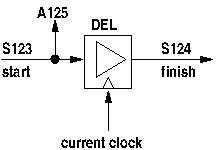
\includegraphics{assert1}
        
        This simplified logic applies if there is no enclosing {\bf priwait()} and hence {\bf pri\_in} and
        {\bf pri\_out} are null. In that case the method could be written as -
        
        \begin{lstlisting}[gobble=8, language=threepl, numbers=left, numberstyle=\tiny, xleftmargin=1cm]
            .
            .  check input and output argument counts
            .
            Ref     oref = outargs.getRef(0, "assert() -");
            if (oref.getMode() != Mode.VALUE)
                throw new ExEx("assert() output argument must be value mode", loc);
            if (oref.getPrimType() != Ptype.LOG)
                throw new ExEx("assert() output argument must be type log", loc);
            
            TDEVar      start = tdelist.signal("S", loc);
            TDEVar      finish = tdelist.signal("S", loc);
            WordSpec    ws = new WordSpec(1, Ptype.LOG);
            TDEVar      tdev = tdelist.signal("A", ws, loc);
            Val         rval = new Val(null, Mode.STATIC, tdev, loc);
            
            rval.addOVar(getCurrentClockVar());
            oref.checkMatch(rval, false, "assert() ", loc);
            oref.assignTo(rval, loc);

            tdelist.connect(tdev, start);

            tdelist.del(finish, start, getCurrentClock(), esig);
            startl.add(start);
            finishl.add(finish);
        \end{lstlisting}
        {\bf oref} is a reference to the output value mode variable.\\
        {\bf start} is a signal we create for the execution thread input.\\
        {\bf finish} is a signal we create which passes on the execution thread.\\
        {\bf ws} is a WordSpec for the assertion output which is type "log".\\
        {\bf tdev} is the assertion output TDEVar with a unique identifier "A.....".\\
        {\bf rval} is a {\bf Val} class wrapper for {\bf tdev}.\\
        
        The assert() call could be enclosed within
        a priwait() in which case instead of simply connecting {\bf tdev} to {\bf start} the following
        would be required -
        
        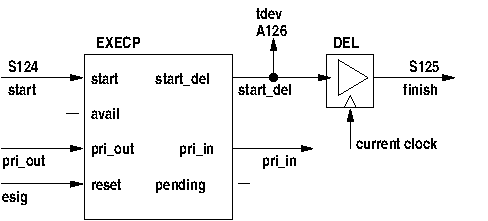
\includegraphics{assert2}
        
        To handle the priwait() an EXECP TDE is required. This can be generated by calling TDEList.execp().
        \begin{lstlisting}[gobble=8, language=java]
            if (pri_in == null)
                tdelist.connect(start_del, start);  // no waitpri
            else {
                TDEVar  v = tdelist.execp(null, start, pri_in, pri_out, esig, null, loc);
                tdelist.connect(start_del, v);
            }
        \end{lstlisting}
        
        
        If in addition we wish to implement the 2nd argument to assert() then an OR gate on the output
        is required -
        
        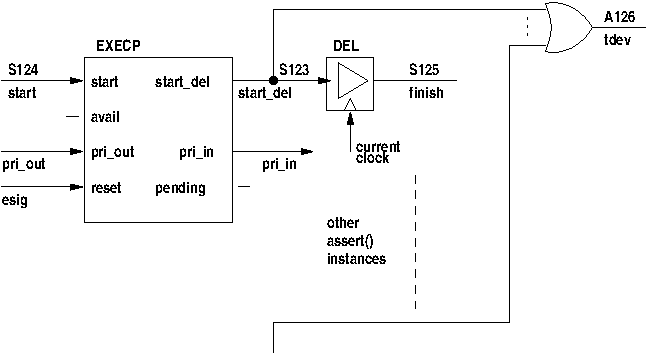
\includegraphics{assert3}

        \begin{lstlisting}[gobble=8, language=java]
            .
            .
            boolean or = false;
            if (inargs.size() == 1) {
                Val     or_val = inargs.getVal(0);
                if (or_val.getMode() != Mode.IMMEDIATE)
                    throw new ExEx("assert() input argument must be immediate mode", loc);
                if (or_val.getPrimType() != Ptype.LOG)
                    throw new ExEx("assert() input argument must be type log", loc);
                or = or_val.getSingleLval(loc);
            }
            .
            .
            if (or) {
                Var     ovar = oref.getVar();
                int     i = oref.getWordSpec().getWord(0);
                if (ovar.getVal(i) == null) {
                    // No initial value so just assign pulse signal.
                    oref.assignTo(rval, loc);
                } else {
                    // Assign OR of initial value and new pulse signal.
                    Val     oval = outargs.getVal(0);
                    TDEVar  otdev = oval.getTDEVar();
                    oref.assignTo(new Val(ovar, Mode.VALUE, tdelist.or(otdev, tdev, loc), loc), loc);
                }
            } else
                oref.assignTo(rval, loc);
            .
            .
        
        \end{lstlisting}
        Note that the previous value of the output argument value mode variable is ORed with the
        assert signal \lstinline[gobble=8, language=java]'tdelist.or(otdev, tdev, loc)'
        Where several assert() statements use the same output argument the assert signals
        will be chained together by ORs. These will later be optimised into a single wide gate
        (TDEList.java optimiseTDEList() line 1199).

